
%\subsectionのタイトルを◯なしに

\section{熊野寮祭 ―これが私たちのやり方だ―}\label{sec:ryosai}
\bunsekisha{文責}{熊野寮祭実行委員会}

\subsecnomaru

 はじめに、皆さんが寮に入る理由には様々なものがあると思います。安いから、コンパとか楽しそうだから、友達がたくさん欲しいから、自治活動をしたいから、、。どれもこれもこの寮の魅力であります。そんな皆さん全員にぜひとも紹介したいのが、年に一度、11月末から12月初めにかけて行われる全寮を挙げたビッグイベント、「熊野寮祭」です。

 補足として、入寮したばかりの新入寮生は、前述の「くまのまつり」と今から述べる「熊野寮祭」をよく混同させてしまうのですが、それぞれ違うお祭りです。「くまのまつり」は、一年のうちで春夏秋の3度行われ、地域の方々に出店していただいたり、ステージに出演していただいたり、一緒に盆踊りを踊ったりと、寮生と地域の方々が織り成すという点で、地域色の濃いお祭りになっています。執筆者自身、「くまのまつり」も大好きなのですが、「熊野寮祭」はそれとはちょっと違うお祭りになります。

 先ほど述べた通り、「熊野寮祭」(以下、寮祭と記す)は、年に一度、11月末から12月初めにかけての10日間で行われます。その規模は、寮内だけに留まらず、京都市、京都府、さらには全国にかけて広がり、「カオスの祭典」とも形容される通り、寮生の考案した企画が各所で乱立するお祭りとなります。2022年度の寮祭では、なんと400もの企画が集まりました。Twitterなどで大きな反響を呼んだ「反ワクチンVS京大生」もこの400のうちの1つです。ここではいくつかの目玉企画をご紹介したいと思います。



\subsection{熊野寮D棟コンパ}

寮祭初日の昼休みにクスノキ前で行われるコンパです。2022年度では、でっかいタテカンを建て、鏡開きとともに寮祭の開幕を高らかに宣言し、ライブしたり、タテカンライブペインティングしたり、おにぎりやサンドウィッチ、さらにはお酒を配ったりしました。このコンパにはキャンパスの学生だけでなく、職員の皆さんも多く詰めかけ、大いに盛り上げてくれます()。「熊野寮D棟」とは、皆さんが時計台と呼んでいる建物のホンモノの名称です。2021年度では「シン・時計台コンパ」という名称でした。



\subsection{エクストリーム帰寮}

参加者は夜中に全国の各所へと飛ばされ、無一文で寮に帰ってくるように命じられます。寮祭が全国規模で行われるとはこういうことです。



\subsection{四条大運動会}

三条河原でのラジオ体操に始まり、早歩き大会、三条ジャンカラ前の広場での騎馬戦、新京極通500mあまりを疾風のごとく南下する二人三脚、借り物競争、四条河原町交差点を舞台とするパン喰い競争、そして四条大橋での大綱引きでフィナーレとなります。ここでは多くの警察が詰めかけ、大いに盛り上げてくれます()。



\subsection{大階段グリコ}

舞台はイルミネーションの輝く京都駅の大階段。そこらへんを歩いている通行人、観光客にじゃんけんを仕掛け、誰よりも速く頂点に登ることを目指します。コミュ力と少しの強運が勝負を左右します。

\subsection{AB棟間綱引き}

寮のA棟とB棟に綱をかけて引き合います。C棟民をいかに仲間にできるかが勝敗を左右します。あおり合戦と稀に起こる裏切りが見所です。

\subsection{鴨川イカダレース}

鴨川を自前のイカダで三条から四条まで南下します。壊れてしまうと極寒の川を泳ぐ羽目になります。


\subsection{}

他にも、演劇、アニメや映画の上映会、種々のコンパ、、。様々な企画が思いつくままに開かれています。個人の単なる思い付きがこの祭では様々な形に変貌します。皆さんの日々の「やってみたい」がこの祭にて実現されます。あなたの企画を寮生は支え、最高に盛り上げ、最高に楽しんでくれます。ここに人の温かみや寮の面白さを再認識し、もっとこの寮のことが好きになるに違いありません。

普段、自分たちの日常が広がる熊野寮が、この期間だけは非日常的な空間へと変貌します。京都大学の学祭、NFが「熊野寮祭の前夜祭」だと称されてしまうほどに、2022年度の寮祭も多くの寮外生を動員し、大変盛り上がりました。また、前述の「くまのまつり」と同様、寮祭パンフに広告を載せるスポンサーになってもらったり、実際に寮祭に遊びに来てもらったりする形で、地域の方々や様々なサークルからのご協力も頂いて、このように毎年大規模に開催することができています。

現在、京都大学は学生の活動に様々な規制をかけています。いわゆる弾圧です。サークルは自由に活動させてもらえず、京大構内や百万遍交差点に設置したタテカンは即撤去され、NFに人数制限がかかり、開かれたお祭りとはなりませんでした。昔できていたことが自由にできなくなってしまったのです。実際、寮祭にも、特に熊野寮D棟コンパや総長室突入など京大構内で実施する企画や、四条大運動会など地域を舞台とする企画には弾圧がかかります。かつては自由に行われていた時計台占拠にも現在では激しい弾圧がかかります。京大が謳っている「自由な学風」は失われつつあるといえます。しかし、そんな中でも熊野寮は長い年月をかけて培ってきた自治を背景に、弾圧に負けることなく企画を貫徹します。京大の自由やカオスとを取り戻すために、私たちはこの祭を全力で盛り上げ、全力で楽しみます。これが私たち熊野寮のやり方です。これが私たち熊野寮の大いなる魅力です。皆さんが京大に求める自由やカオスはここにあります。皆さんも私たちと一緒にそれを体現しましょう!次なる主役は君たちだ!


\begin{figure}[H]
  \centering
  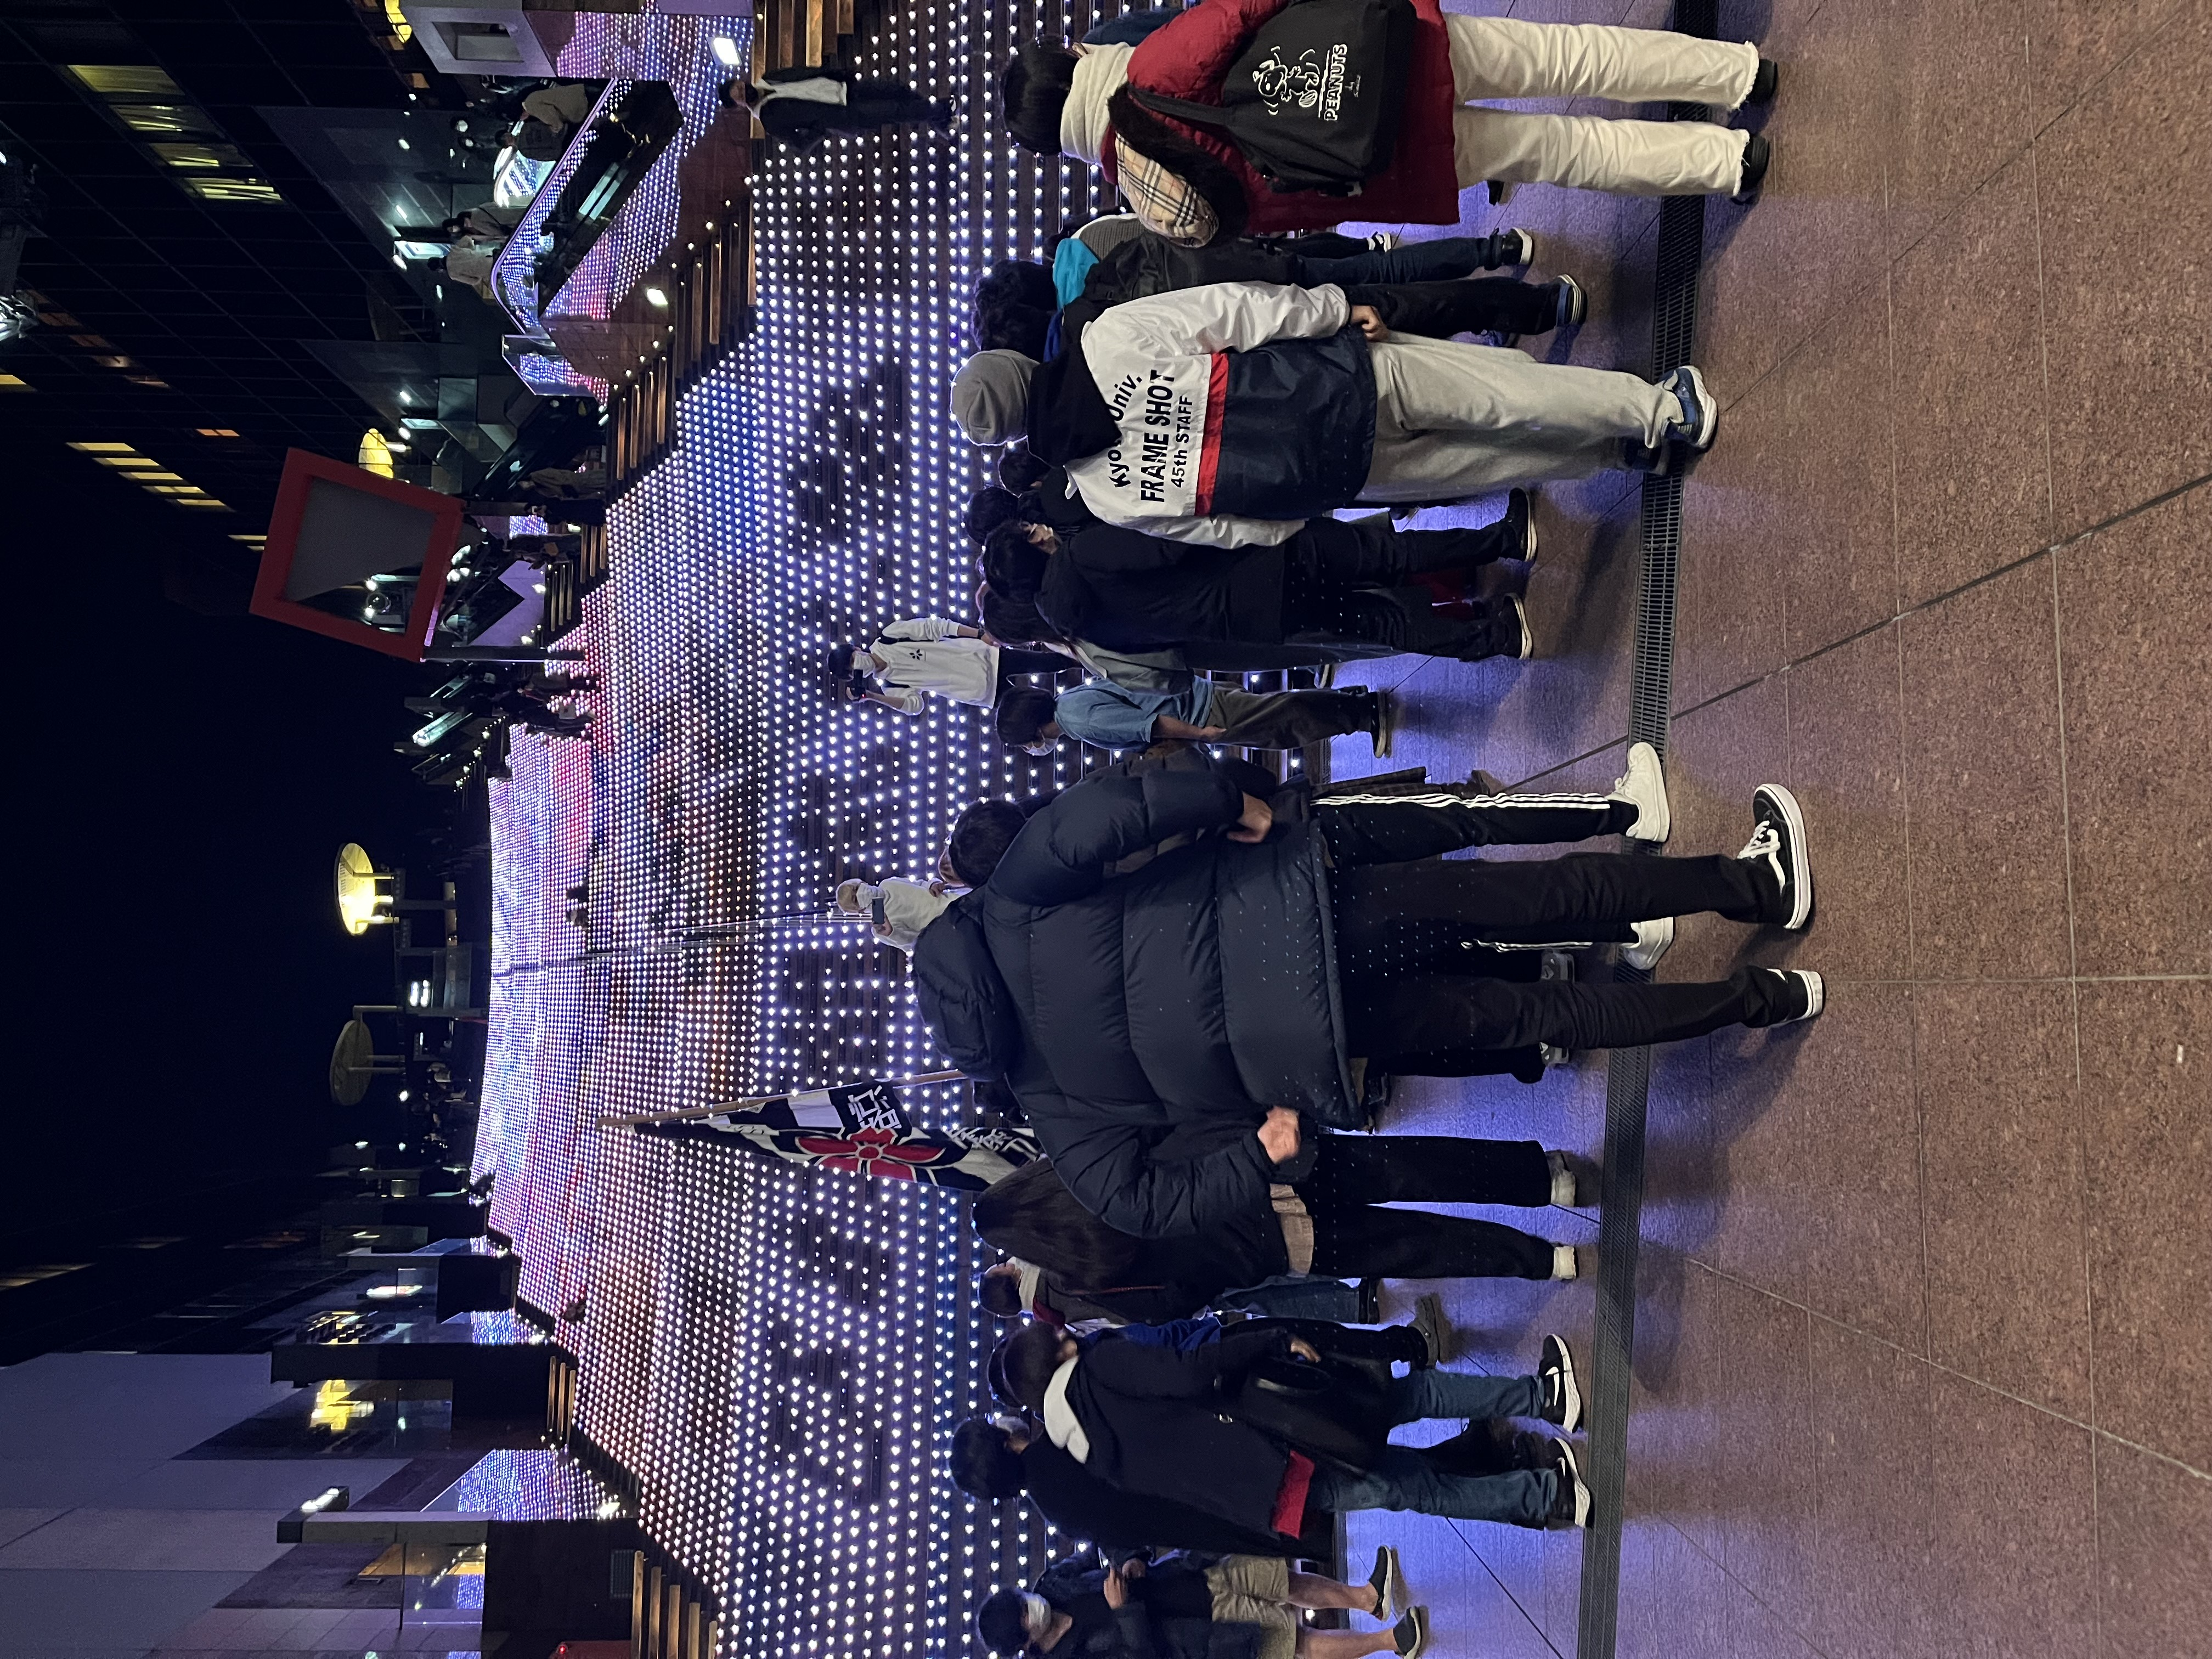
\includegraphics[height=5cm, angle=-90]{gazo/guriko.jpg}%何故か横倒しになるので、angleオプションを付けている。
  \subcaption{{\small 京都駅大階段グリコ}}
  
\end{figure}

\subsecdefault
%\subsectionのデザインを元に戻す



